\documentclass{article}
\usepackage[margin=1in]{geometry}
\usepackage{amsmath,amsthm,amssymb}
\usepackage{bbm,enumerate,mathtools}
\usepackage{tikz,pgfplots}
\usepackage{chessboard}
\usepackage[hidelinks]{hyperref}
\usepackage{multicol} % Problem 35

\newenvironment{question}{\begin{trivlist}\item[\textbf{Question.}]}{\end{trivlist}}
\newenvironment{note}{\begin{trivlist}\item[\textbf{Note.}]}{\end{trivlist}}
\newenvironment{references}{\begin{trivlist}\item[\textbf{References.}]}{\end{trivlist}}
\newenvironment{related}{\begin{trivlist}\item[\textbf{Related.}]\end{trivlist}\begin{enumerate}}{\end{enumerate}}


\begin{document}
\rating{2}{2}
According to Peter Winkler's problem ``Red and Blue Dice'' in
\textit{Mathematical Mind-Benders}, given two sequences of length $n$ with
letters in $[n]$, there must always exist a (nonempty) subsequence in each such
that the sum of each of the subsequences are equal.
Furthermore, there must exist a \textit{substring} (i.e. contiguous subset) in
both such that the sum of each substring is equal.
\begin{figure}[ht!]
  \centering
  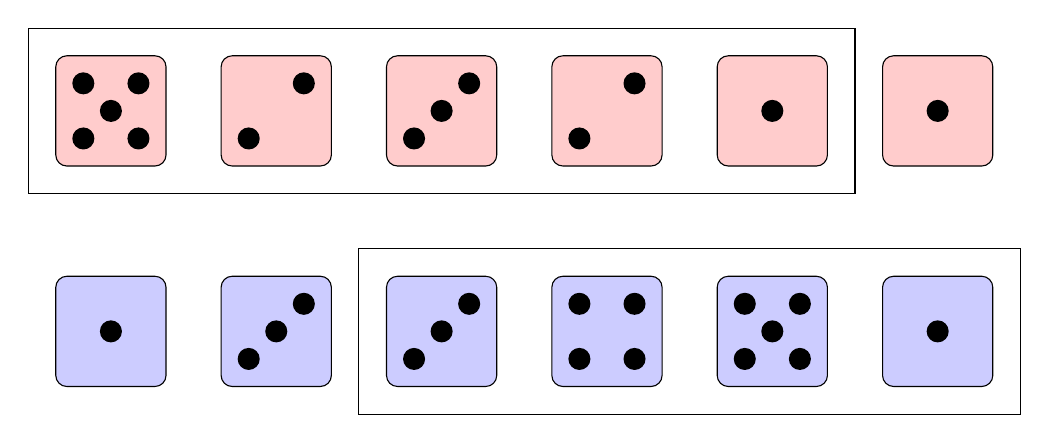
\begin{tikzpicture}[scale=0.7]
    \foreach \i in {0,3,6,9,12,15} {
      \draw[rounded corners, fill=red!20] (\i,4) rectangle (\i + 2,6);
      \draw[rounded corners, fill=blue!20] (\i,0) rectangle (\i + 2,2);
    }
    \fill (1,5) circle (0.2)
          (0.5,4.5) circle (0.2)
          (1.5,4.5) circle (0.2)
          (0.5,5.5) circle (0.2)
          (1.5,5.5) circle (0.2);
    \fill (3.5,4.5) circle (0.2)
          (4.5,5.5) circle (0.2);
    \fill (6.5,4.5) circle (0.2)
          (7,5) circle (0.2)
          (7.5,5.5) circle (0.2);
    \fill (9.5,4.5) circle (0.2)
          (10.5,5.5) circle (0.2);
    \fill (13,5) circle (0.2);
    \fill (16,5) circle (0.2);

    \fill (1,1) circle (0.2);
    \fill (3.5,0.5) circle (0.2)
          (4,1) circle (0.2)
          (4.5,1.5) circle (0.2);
    \fill (6.5,0.5) circle (0.2)
          (7,1) circle (0.2)
          (7.5,1.5) circle (0.2);
    \fill (9.5,0.5) circle (0.2)
          (10.5,0.5) circle (0.2)
          (9.5,1.5) circle (0.2)
          (10.5,1.5) circle (0.2);
    \fill (13,1) circle (0.2)
          (12.5,0.5) circle (0.2)
          (13.5,0.5) circle (0.2)
          (12.5,1.5) circle (0.2)
          (13.5,1.5) circle (0.2);
    \fill (16,1) circle (0.2);
    \draw (-0.5,3.5) rectangle (14.5, 6.5);
    \draw (5.5,-0.5) rectangle (17.5, 2.5);
  \end{tikzpicture}
  \caption{
    The first five dice in the top row have the same sum as the last four dice
    in the bottom row.
  }
\end{figure}

\begin{question}
  How many equal-sum subsequences (respectively substrings) are guaranteed to
  exist?
\end{question}

\begin{related}
  \item What if the subsequence or substring must have length greater than or
    equal to $k$?
  \item What if the subsequences or substrings must be of equal length?
  \item What if the substring is allowed to wrap around?
  \item What if this is done over permutations $S_n$ instead of subsets $[n]^n$?
  \item What if the sequences are of length $\ell < n$, and must be injections
  from $\mathbb N$ to $[n]$?
  \item What if there are three sequences? $m$ sequences?
  \item Given two random sequences, what is the expected number of equal-sum
  subsequences?
\end{related}


\begin{references}
  \item \url{https://math.stackexchange.com/q/3035452/121988}
\end{references}

\end{document}
